% Mecánico rotacional: par de engranajes
\documentclass[border=5pt]{standalone}
\usepackage{tikz}
\usetikzlibrary{arrows.meta}
\begin{document}
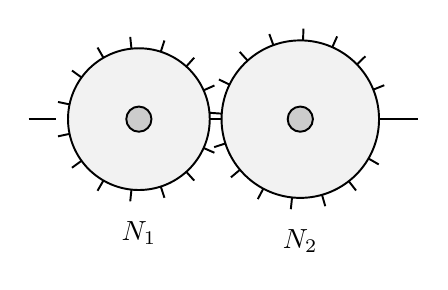
\begin{tikzpicture}[line width=0.7pt]
  % engranaje 1 (centro 0,0 radio 0.9)
  \foreach \a in {0,24,...,336} \draw (\a:0.9) -- (\a:1.05);
  \draw[fill=black!5] (0,0) circle (0.9);
  \draw[fill=black!20] (0,0) circle (0.16);
  \node at (0,-1.45) {$N_1$};
  % engranaje 2 (centro 2.05,0 radio 1.0; dist = 0.9+1.0 + holgura)
  \foreach \a in {0,22,...,338} \draw ([shift={(2.05,0)}]\a:1.0) -- ([shift={(2.05,0)}]\a:1.15);
  \draw[fill=black!5] (2.05,0) circle (1.0);
  \draw[fill=black!20] (2.05,0) circle (0.16);
  \node at (2.05,-1.55) {$N_2$};
  % ejes
  \draw (-1.4,0) -- (-1.05,0);
  \draw (3.2,0) -- (3.55,0);
\end{tikzpicture}
\end{document}
